\section{SiD vertex detector occupancies}
The occupancy of the SiD vertex detector is calculated by counting the hits from the pair background per pixel for a full bunch train (1312 bunch crossings).
The sensor buffers are read out after every train, and therefore have to be suitable for the expected detector occupancy.
For the study of the occupancy, the pair background events were taken from GuineaPig, as described in the section before, and used as input for a full Geant4 detector simulation with SLIC~\cite{SLIC}.
The crossing angle was applied in this simulation step.\\
Regarding the SiD detector geometry, a pixel size of 20x\SI{20}{\micro\meter} was assumed for the vertex detector.
The SiD vertex detector is a high-resolution pixel detector with the following requirements:
\begin{itemize}
 \item Spatial resolution: $<$ \SI{4}{\micro\meter}
 \item Momentum resolution: $\sim$ 2-\SI{5e-5}{\GeV}
 \item $\sim$ \SI{0.1}{\percent} X\textsubscript{0} per layer
\end{itemize}
Table~\ref{tab:KeyParametersSiD} lists further key parameters and measurements of the vertex detector, for which a visualization is shown in Figure~\ref{fig:SiD}.
\begin{table}[h]
\caption{\textit{Key design parameters of the baseline SiD vertex detector (VXD). All dimensions are given in cm.}}
\label{tab:KeyParametersSiD}
\centering
\begin{tabularx}{\textwidth}{l|llll}
\hline\hline
& Technology & Inner radius & Outer radius & z extent\\
\hline
VXD barrel & Silicon pixels & 1.4 & 6.0 & $\pm 6.25$ \\
\hline\hline
& Technology & Inner z & Outer z & Outer radius\\
\hline
VXD endcap & Silicon pixels & 7.3 & 83.4 & 16.6 \\
\hline\hline
\end{tabularx}
\end{table}

\begin{figure}[!h]
\centering
\begin{subfigure}[t]{0.45\textwidth}
\centering
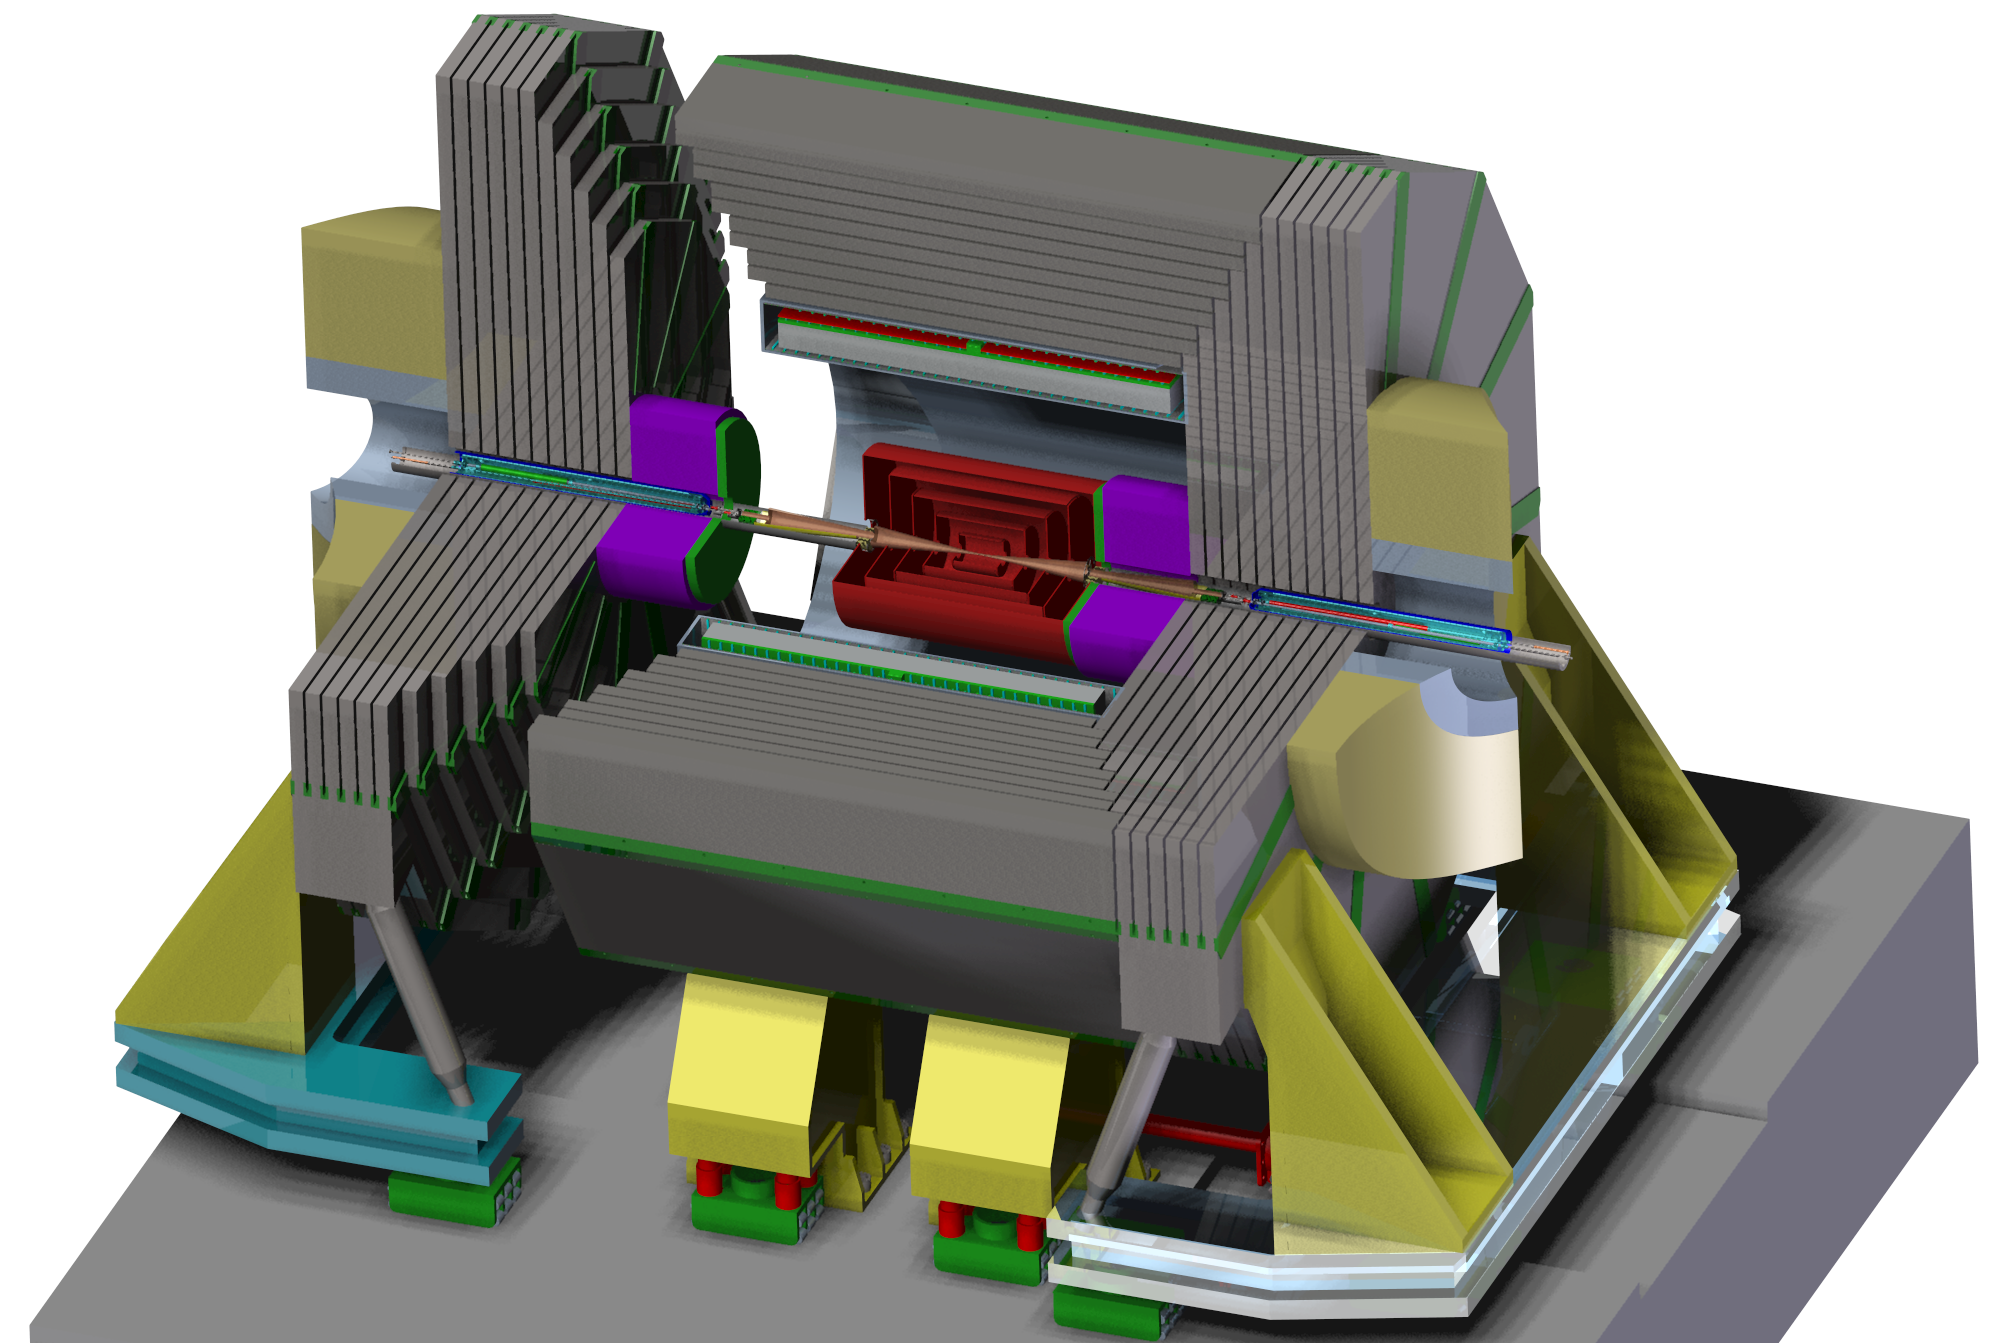
\includegraphics[width=1.05\textwidth]{figures/SiD_new.png}
\caption{\textit{Visualization of the full SiD detector}}
\end{subfigure}
\hspace*{0.3cm}
\begin{subfigure}[t]{0.45\textwidth}
\centering
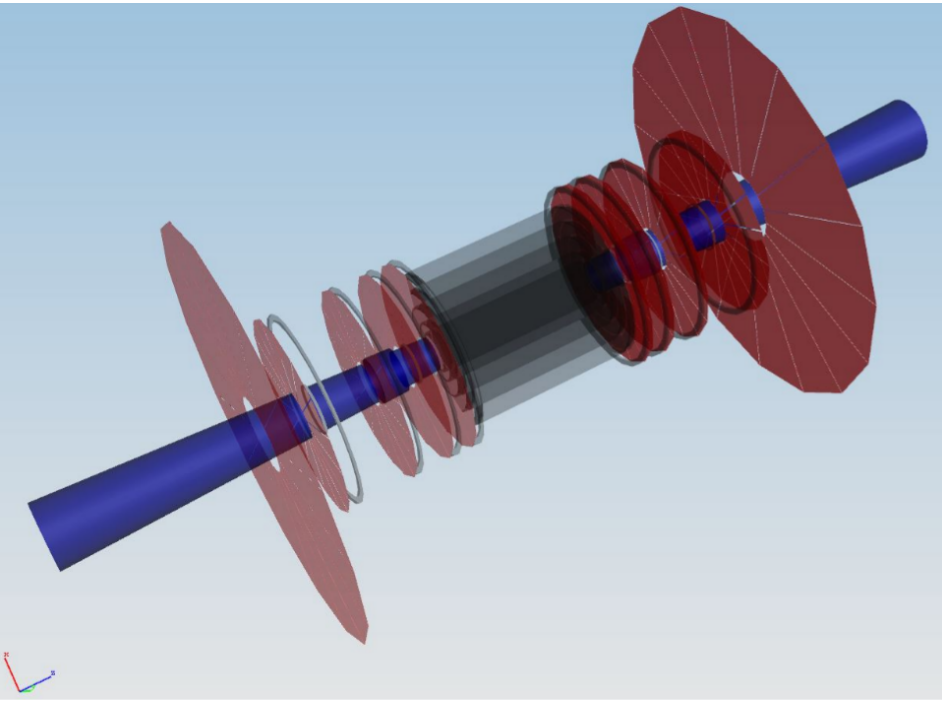
\includegraphics[width=1.05\textwidth]{figures/SiDVertexDetector.png}
\caption{\textit{Visualization of the SiD vertex detector}}
\end{subfigure}
\caption{\textit{Visualizations of the current design models of the SiD detector (a), and the SiD vertex detector (b).}}
\label{fig:SiD}
\end{figure}

\subsection{Occupancy studies for the current SiD design}
The current SiD design with an L$^*$ of \SI{4.1}{\meter} (the distance between the interaction point and the last quadrupole magnet of the Final-Focus system) foresees an anti-DiD magnet with a magnetic field strength of \SI{600}{\gauss}.
It reduces the pair background occupancy by sweeping the pair background particles through the outgoing beam pipe.
The following plots show occupancy studies using the current SiD geometry.\\
On the left hand side of Figure~\ref{fig:All_layers_Occupancy}, the normalized occupancy for the full vertex detector is shown.
From that, the ratio of dead cells was calculated (right).
A cell is "dead" when the number of hits in this cell has reached the cell's buffer depth.
Therefore, the number of dead cells is plotted as a function of the assumed buffer depth for the vertex detector cells.
For all layers combined, the new parameter scheme (A) leads to a fraction of dead cells that is 2-3 times higher than for the TDR set.
Again, for the other schemes (B) and (C), the fraction is even higher.
\begin{figure}[!h]
\centering
\begin{subfigure}[t]{0.45\textwidth}
\centering
\includegraphics[width=1.05\textwidth]{figures/Occupancy_Comparison_All_layers_wrt_cells_ILC250_Comparison_ALL_SETS_5T_w_antiDiD.png}
\caption{\textit{Normalized Occupancy:\\Number of cells containing a certain amount of hits, normalized by the total number of cells of the vertex detector.}}
\end{subfigure}
\hspace*{0.3cm}
\begin{subfigure}[t]{0.45\textwidth}
\centering
\includegraphics[width=1.05\textwidth]{figures/Occupancy_Comparison_All_layers_deadcells_ILC250_Comparison_ALL_SETS_5T_w_antiDiD.png}
\caption{\textit{Ratio of dead cells in comparison to all cells of the vertex detector.}}
\end{subfigure}
\caption{\textit{Pair background occupancy in the SiD vertex detector for all vertex detector layers combined.}}
\label{fig:All_layers_Occupancy}
\end{figure}
\\In general, the occupancy in layer 0 is higher than in the other layers, as it is the layer closest to the interaction point.
Here, the occupancy for the new sets is significantly increased with respect to the TDR scheme (see Figure~\ref{fig:Layer0_Occupancy}). 
\begin{figure}[!h]
\centering
\begin{subfigure}[t]{0.45\textwidth}
\centering
\includegraphics[width=1.05\textwidth]{figures/Occupancy_Comparison_Layer_0_numcells_ILC250_Comparison_ALL_SETS_5T_w_antiDiD.png}
\caption{\textit{Layer 0: Normalized Occumancy}}
\end{subfigure}
\hspace*{0.3cm}
\begin{subfigure}[t]{0.45\textwidth}
\centering
\includegraphics[width=1.05\textwidth]{figures/Occupancy_Comparison_Layer_0_deadcells_ILC250_Comparison_ALL_SETS_5T_w_antiDiD.png}
\caption{\textit{Layer 0: Ratio of dead cells}}
\end{subfigure}
\caption{\textit{Pair background occupancy in the SiD vertex detector layer 0.
The plots on the left hand side show the normalized occupancy, the ratio of dead cells is shown on the right side.}}
\label{fig:Layer0_Occupancy}
\end{figure}

\subsection{Occupancy studies as a comparison of different SiD designs}
In the following, different SiD designs are compared by observing the vertex detector occupancy for the new ILC250 parameter set (A).
The studied designs are different combinations of the old L$^*$ value (\SI{3.5}{\meter}) vs. the new value, and of the inclusion or exclusion of the anti-DiD field.
Again, the normalized occupancy is plotted for all vertex detector layers combined, as well as only for layer 0 (see Figure~\ref{fig:SiD_comparison}).
\begin{figure}[!h]
\centering
\begin{subfigure}[t]{0.45\textwidth}
\centering
\includegraphics[width=1.05\textwidth]{figures/Occupancy_Comparison_All_layers_wrt_cells_ILC250_Comparison_SET_A_5T_different_SiD_geometries.png}
\caption{\textit{All layers combined}}
\end{subfigure}
\hspace*{0.3cm}
\begin{subfigure}[t]{0.45\textwidth}
\centering
\includegraphics[width=1.05\textwidth]{figures/Occupancy_Comparison_Layer_0_numcells_ILC250_Comparison_SET_A_5T_different_SiD_geometries.png}
\caption{\textit{Layer 0}}
\end{subfigure}
\caption{\textit{Pair background occupancy in the SiD vertex detector for different SiD designs.
The plot on the left hand side shows the normalized occupancy for all layers combined, whilst the normalized occupancy for only layer 0 is shown on the right.}}
\label{fig:SiD_comparison}
\end{figure}
\\Figure~\ref{fig:SiD_comparison} shows that the SiD design does not have a big impact on the vertex detector occupancy from the pair background. 
The lowest occupancy is reached for the SiD design with the old L$^*$ and anti-DiD.\\
However, the current SiD design (new L$^*$ with anti-DiD) shows occupancy levels that are only marginally worse.
Assuming a buffer depth of four, just above 10$^{-5}$ of all cells in layer 0 would have full buffers, filled with exactly 4 hits.
With the rule of thomb that the vertex detector occupancy for backgrounds should be below 10$^{-4}$, the occupancies for all studies shown in this note are well below this boundary.